
% TABLES:


\nopagebreak[0]

%late after line=\\\hline,
\begin{table}[H]
	\catcode`"=9
	\caption{\small Range of Observation Periods for each Country }
	%	\vspace{-20pt}
	\label{tab:app_data_countryrange}
	{\tiny{
			\newcolumntype{Y}{>{\centering\arraybackslash}X}
			\begin{tabularx}{\textwidth}{l l Y Y }\toprule
				%& & \multicolumn{2}{c}{\textbf{Forecasts}}  & \multicolumn{2}{c}{\textbf{Actual Outcomes}}   \\
				& \textbf{Country} & \textbf{GDP} & \textbf{CPI}  \\ \hline \midrule
				\csvreader[
				late after line=\\,
				late after last line=\\\bottomrule]
				{Sections/countryTimeVar.csv}{country=\country,fdGdpCurrent=\fdGdpCurrent,ldGdpCurrent=\ldGdpCurrent,fdCpiCurrent=\fdCpiCurrent,ldCpiCurrent=\ldCpiCurrent}%
				{\thecsvrow & \country& \fdGdpCurrent  -- ~\ldGdpCurrent & \fdCpiCurrent  -- ~\ldCpiCurrent }%
			\end{tabularx}
		}
	}
	\centering	
	
	\begin{minipage}{1\textwidth}
		
		\begin{tabnote}
			\textit{Notes:}  The table shows the first and last observation date for GDP and CPI for which forecasts and vintages are available. The data for forecasts come from Consensus Economics, while actual outcomes are from the International Monetary Fund World Economic Outlook (IMF WEO).
		\end{tabnote}
	\end{minipage}
\end{table}






%
%\begin{table}
%	\catcode`"=9
%	\caption{\small Range of Observation Periods for each Country }
%	%	\vspace{-20pt}
%	\label{tab:app_data_countryrange2}
%	{\tiny{
%			\newcolumntype{Y}{>{\centering\arraybackslash}X}
%			\begin{tabularx}{\textwidth}{l l Y Y l l Y Y}\toprule
%				%& & \multicolumn{2}{c}{\textbf{Forecasts}}  & \multicolumn{2}{c}{\textbf{Actual Outcomes}}   \\
%				& \textbf{Country} & \textbf{CPI} & \textbf{GDP} & & \textbf{Country} & \textbf{CPI} & \textbf{GDP}  \\ \hline \midrule
%				\csvreader[
%				late after line=\\,
%				late after last line=\\\bottomrule]
%				{Sections/countryTimeVarOnlyFC_2col.csv}{
%					n = \n,
%					country=\country,
%					fdCpiCurrent=\fdCpiCurrent,
%					ldCpiCurrent=\ldCpiCurrent,
%					fdGdpCurrent=\fdGdpCurrent,
%					ldGdpCurrent=\ldGdpCurrent,
%					nb = \nb,
%					countryb=\countryb,
%					fdCpiCurrentb=\fdCpiCurrentb,
%					ldCpiCurrentb=\ldCpiCurrentb,
%					fdGdpCurrentb=\fdGdpCurrentb,
%					ldGdpCurrentb=\ldGdpCurrentb
%		}%
%				{\n & \country& 
%					\fdGdpCurrent  -- ~\ldGdpCurrent & 
%					\fdCpiCurrent  -- ~\ldCpiCurrent  &
%					\nb & \countryb& 
%					\fdGdpCurrentb  -- ~\ldGdpCurrentb & 
%					\fdCpiCurrentb  -- ~\ldCpiCurrentb  
%		}%
%			\end{tabularx}
%		}
%	}
%	\centering	
%	
%	\begin{minipage}{1\textwidth}
%		
%		\begin{tabnote}
%			\textit{Notes:}  The table shows the first and last observation date for CPI and GDP for which forecasts and vintages are available. The data for forecasts comes from Consensus Economics, while actual outcomes are from the International Monetary Fund World Economic Outlook (IMF WEO).
%		\end{tabnote}
%	\end{minipage}
%\end{table}





\input{Tables/emerging_developed_sum}


%late after line=\\\hline,

% Below, the table includes dates for vintages. But since we drop forecasts (vintages) when vintages (forecasts) are not available, the information is redundent.
%\begin{table}
%	\catcode`"=9
%	\caption{\small Range of Observation Periods for each Country }
%	%	\vspace{-20pt}
%	\label{tab:app_data_countryrange}
%	{\scriptsize{
		%			\newcolumntype{Y}{>{\centering\arraybackslash}X}
		%			\begin{tabularx}{\textwidth}{l l Y Y Y Y}\toprule
			%				& & \multicolumn{2}{c}{\textbf{Forecasts}}  & \multicolumn{2}{c}{\textbf{Actual Outcomes}}   \\
			%				& \textbf{Country} & \textbf{GDP} & \textbf{CPI}& \textbf{GDP} & \textbf{CPI} \\ \hline \midrule
			%				\csvreader[
			%				late after line=\\,
			%				late after last line=\\\bottomrule]
			%				{Sections/countryTimeVar.csv}{country=\country,fdGdpCurrent=\fdGdpCurrent,ldGdpCurrent=\ldGdpCurrent,fdCpiCurrent=\fdCpiCurrent,ldCpiCurrent=\ldCpiCurrent,fdVintageGdpCurrent=\fdVintageGdpCurrent,ldVintageGdpCurrent=\ldVintageGdpCurrent,fdVintageCpiCurrent=\fdVintageCpiCurrent,ldVintageCpiCurrent=\ldVintageCpiCurrent}%
			%				{\thecsvrow & \country& \fdGdpCurrent  -- ~\ldGdpCurrent & \fdCpiCurrent  -- ~\ldCpiCurrent & \fdVintageGdpCurrent  -- ~\ldVintageGdpCurrent & \fdVintageCpiCurrent  $-$  ~\ldVintageCpiCurrent}%
			%			\end{tabularx}
		%		}
	%	}
%	\centering	
%	
%	\begin{minipage}{1\textwidth}
	%		
	%		\begin{tabnote}
		%			\textit{Notes:}  The table shows the first and last observation date for GDP and CPI and for forecasts as well as for the actual outcomes. The data for forecasts comes from Consensus Economics, while actual outcomes are from the International Monetary Fund World Economic Outlook (IMF WEO).
		%		\end{tabnote}
	%	\end{minipage}
%\end{table}

\begin{figure}[h]
		\centering
		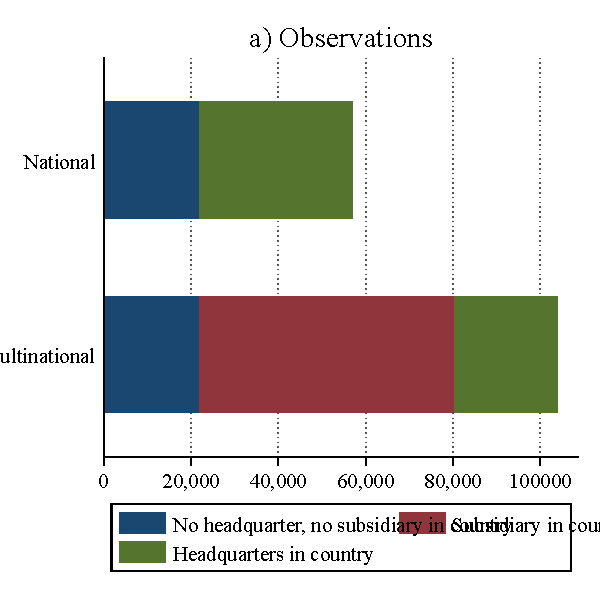
\includegraphics[width=.45\linewidth]{Figures/hq_sub_obs.pdf}
		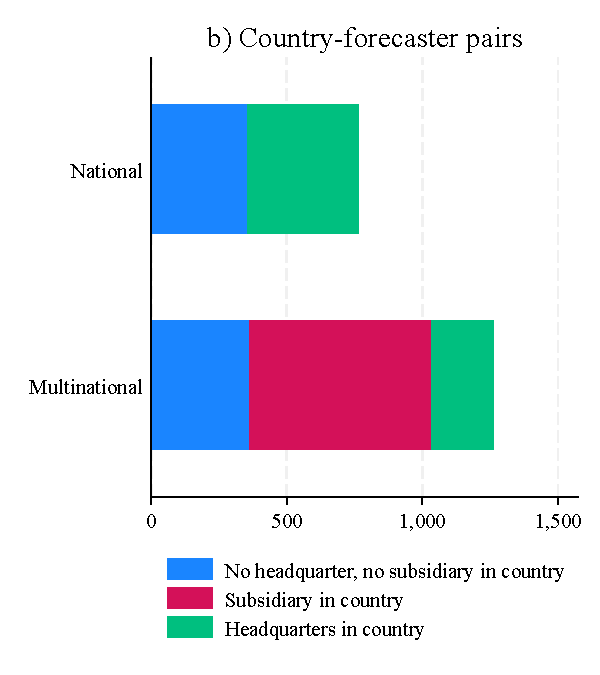
\includegraphics[width=.45\linewidth]{Figures/hq_sub_pairs.pdf}
	\caption{Distribution of forecasts and country-forecaster pairs conditional on Location and Scope of Forecaster}
	\label{fig:hq_sub_obs}
	\begin{fignote}
		\textit{Notes:} The figure shows the distribution of the forecasts and country-forecaster pairs conditional on the location and scope of the forecaster. A forecast is either provided by a forecaster with headquarters located in the country, or by a forecaster with no headquarters but with at least a subsidiary located in the country, or by a forecaster with neither headquarters or subsidiaries located in the country. Multinational forecasters have subsidiaries in countries other than the one where their headquarters are located. National forecasters have only subsidiaries in the same country as their headquarters.
	\end{fignote}
\end{figure}

\begin{figure}[h]
		\centering
		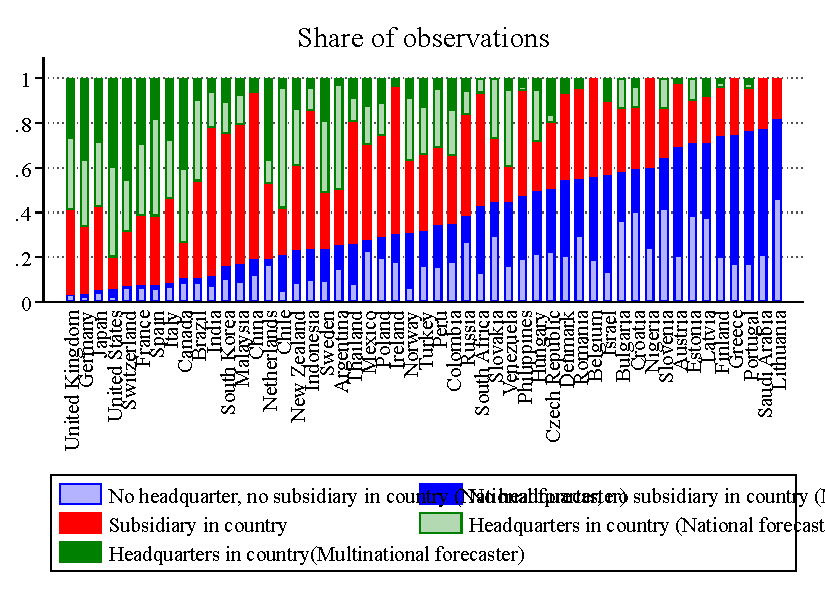
\includegraphics[width=1\linewidth]{Figures/hq_sub_obs_by_cty.pdf}
	\caption{Proportion of forecasts conditional on Location and Scope of Forecaster, by country}
	\label{fig:hq_sub_obs_by_cty}
	\begin{fignote}
		\textit{Notes:} The figure shows the distribution of the forecasts conditional on the location and scope of the forecaster. A forecast is either provided by a forecaster with headquarters located in the country, or by a forecaster with no headquarters but with at least a subsidiary located in the country, or by a forecaster with neither headquarters or subsidiaries located in the country. Multinational forecasters have subsidiaries in countries other than the one where their headquarters are located. National forecasters have only subsidiaries in the same country as their headquarters.
	\end{fignote}
\end{figure}

\begin{figure}[h]
		\centering
		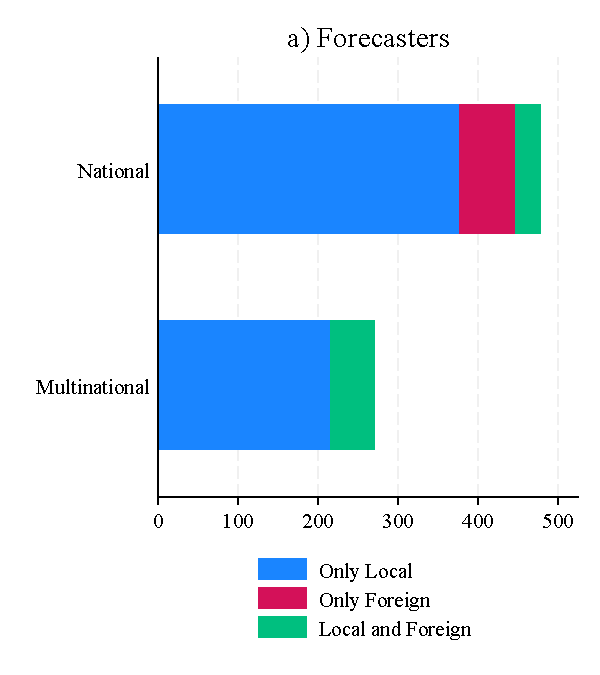
\includegraphics[width=.45\linewidth]{Figures/loc_for_inst.pdf}
		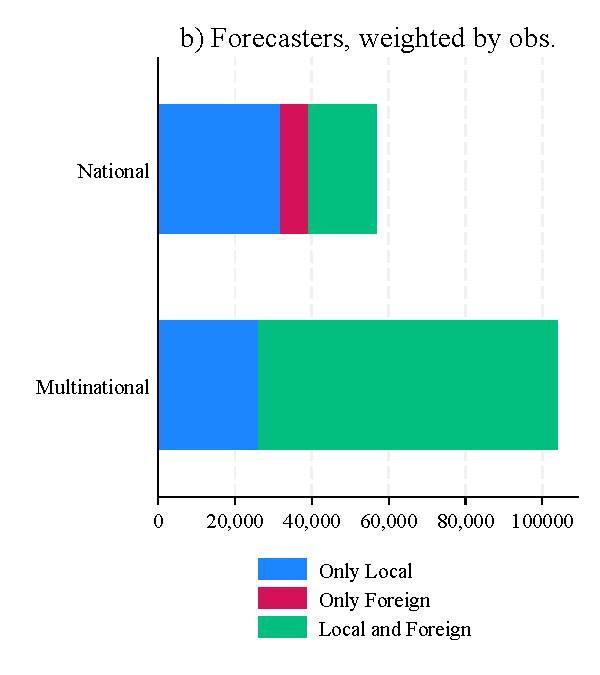
\includegraphics[width=.45\linewidth]{Figures/loc_for_obs.pdf}	
	\caption{Forecasters publishing Local and Foreign Forecasts}
	\label{fig:loc_for}
	\begin{fignote}
		\textit{Notes:} The figure shows the distribution of the forecasters depending on the nature of their forecasts. A forecaster either provides local forecasts only, or foreign forecasts only, or both local and foreign forecasts.
	\end{fignote}
\end{figure}

\begin{figure}[h]
		\centering
		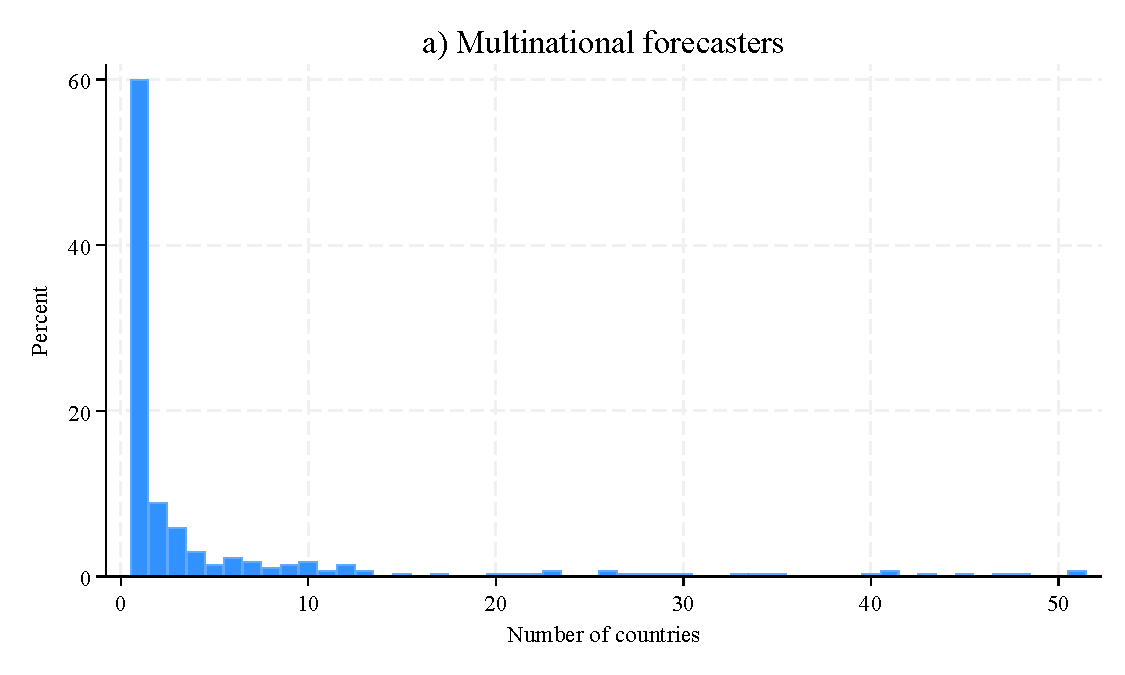
\includegraphics[width=.45\linewidth]{Figures/hist_mult.pdf}
		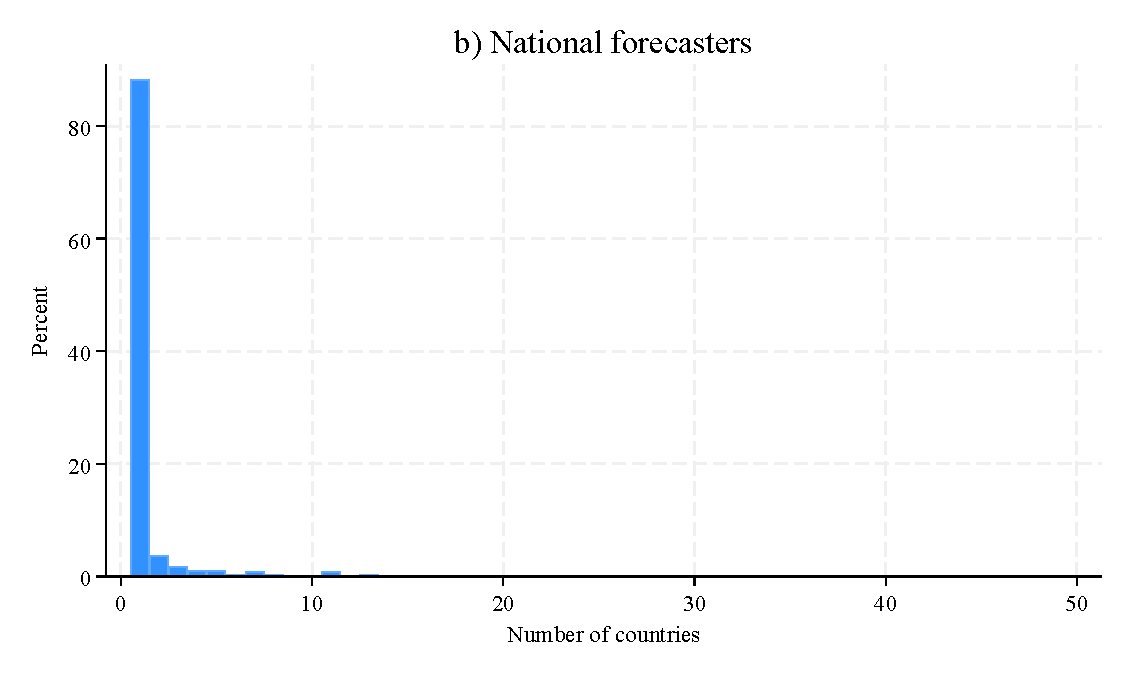
\includegraphics[width=.45\linewidth]{Figures/hist_nat.pdf}	
	\caption{Number of countries in forecasters' portfolio}
	\label{fig:hist}
	\begin{fignote}
		\textit{Notes:} The figure shows the distribution, across forecasters, of the number of countries that are in a forecaster's portfolio, depending of the forecaster's scope (multinational or national firm). A country is in a forecaster's portfolio if the forecaster provides forecasts for that country.
	\end{fignote}
\end{figure}